\documentclass[12pt,a4]{article}
\usepackage{physics, amsmath,amsfonts,amsthm,amssymb, mathtools,steinmetz, gensymb, siunitx}	% LOADS USEFUL MATH STUFF
\usepackage{xcolor,graphicx}
\usepackage{caption}
\usepackage{subcaption}
\usepackage[left=45pt, top=20pt, right=45pt, bottom=45pt ,a4paper]{geometry} 				% ADJUSTS PAGE
\usepackage{setspace}
\usepackage{tikz}
\usepackage{pgf,tikz,pgfplots,wrapfig}
\usepackage{mathrsfs}
\usepackage{fancyhdr}
\usepackage{float}
\usepackage{array}
\usepackage{booktabs,multirow}
\usepackage{bm}
\usepackage{tensor}
\usepackage{listings}
 \lstset{
    basicstyle=\ttfamily\small,
    numberstyle=\footnotesize,
    numbers=left,
    backgroundcolor=\color{gray!10},
    frame=single,
    tabsize=2,
    rulecolor=\color{black!30},
    title=\lstname,
    escapeinside={\%*}{*)},
    breaklines=true,
    breakatwhitespace=true,
    framextopmargin=2pt,
    framexbottommargin=2pt,
    inputencoding=utf8,
    extendedchars=true,
    literate={á}{{$\rho$}}1 {ã}{{\~a}}1 {é}{{\'e}}1,
}
\DeclareMathOperator{\sign}{sgn}
\DeclareMathOperator{\arcosh}{arcosh}
\DeclareMathOperator{\arsinh}{arsinh}
\DeclareMathOperator{\artanh}{artanh}
\DeclareMathOperator{\arsech}{arsech}
\DeclareMathOperator{\arcsch}{arcsch}
\DeclareMathOperator{\arcoth}{arcoth} 

\usetikzlibrary{decorations.text, calc}
\pgfplotsset{compat=1.7}

\usetikzlibrary{decorations.pathreplacing,decorations.markings}
\usepgfplotslibrary{fillbetween}

\newcommand{\vect}[1]{\boldsymbol{#1}}

\usepackage{hyperref}

%\usepackage[style= ACM-Reference-Format, maxbibnames=6, minnames=1,maxnames = 1]{biblatex}
%\addbibresource{references.bib}


\hypersetup{pdfborder={0 0 0},colorlinks=true,linkcolor=black,urlcolor=cyan,}
\allowdisplaybreaks
%\hypersetup{
%
%    colorlinks=true,
%
%    linkcolor=blue,
%
%    filecolor=magenta,      
%
%    urlcolor=cyan,
%
%    pdftitle={An Example},
%
%    pdfpagemode=FullScreen,
%
%    }
%}

\title{
\textsc{Statistical Physics Homework 2}
}
\author{\textsc{J L Gouws}
}
\date{\today
\\[1cm]}



\usepackage{graphicx}
\usepackage{array}




\begin{document}
\thispagestyle{empty}

\maketitle

\begin{enumerate}
  \item
    \begin{enumerate}
      \item
        Taking the inverse fourier transform of the elements of $B$ gives:
        \begin{align*}
          \sum_j B_{ij} 
%                        &= \sum_{j}\frac{1}{N} \sum_k B_k e^{i k \cdot (x_i - x_j)}\\
%                        &= \frac{1}{N} \sum_k B_k  e^{i k \cdot x_i} \sum_{j} e^{-i k \cdot x_j)}
                        &= \sum_{j}  \frac{1}{N^2} \sum_{k q} \hat B_{kq} e^{i k \cdot x_i} e^{i q \cdot x_i}
        \end{align*}
        Assuming that the model is limited to nearest neighbour interactions:
        \begin{align*}
          \sum_j B_{ij} 
                        &= \sum_{j}  \frac{1}{N^2} \sum_{k q} N B_k \delta_{k + q, 0} e^{i k \cdot x_i} e^{i q \cdot x_j}\\
                        &=   \frac{1}{N^2} \sum_{k q} N B_k \delta_{k + q, 0} e^{i k \cdot x_i} \sum_{j} e^{i q \cdot x_j}\\
                        &=   \frac{1}{N^2} \sum_{k q} N B_k \delta_{k + q, 0} e^{i k \cdot x_i} N \delta_{q,0}\\
                        &=   \frac{1}{N^2} \sum_{k} N^2 B_k \delta_{k, 0} e^{i k \cdot x_i} \\
                        &=   B_0 
        \end{align*}
      \item
        For the minimum, derivatives are taken:
        \begin{align*}
          \frac{\partial S}{\partial \phi_i} &= \frac{\partial }{\partial \phi_i}\left(\frac{\beta A^2}{2} \phi^T B \phi - \sum_j \ln(\cosh(\beta A (B \phi)_j))\right)\\
                                             &= \frac{\beta A^2}{2} \frac{\partial }{\partial \phi_i}\sum_{ij}\phi_i B_{ij} \phi_j - \frac{\partial }{\partial \phi_i}\sum_j \ln(\cosh(\beta A (B \phi)_j))\\
                                             &= \frac{\beta A^2}{2} \sum_{j} \left( B_{ij} \phi_j + \phi_jB_{ji} \right) - \sum_j \beta A B_{ji}\frac{\sinh(\beta A (B \phi)_j)}{\cosh(\beta A (B \phi)_j)}\\
                                             &= \frac{\beta A^2}{2} \sum_{j} \left( B_{ij} \phi_j + \phi_jB_{ji} \right) - \beta A\sum_j B_{ji}\tanh(\beta A (B \phi)_j)\\
                                             &= \beta A^2 \sum_{j} B_{ij} \phi_j - \beta A \sum_j B_{ji}\tanh(\beta A (B \phi)_j)
        \end{align*}
        This is zero at the critical point $\psi_i = \bar{\psi}$ for every $i$, and evaluating for very $i$ gives the result:
        \begin{align*}
          0 = \left.\frac{\partial S}{\partial \phi_i}\right|_{\phi_i = \bar{psi}} 
                                             &= \beta A^2 \sum_{j} B_{ij} \phi_{j} - \beta A \sum_j B_{ji}\tanh(\beta A \sum_k B_{jk} \phi_k)\\
                                             &= \beta A^2 \sum_{j} B_{ij} \bar{\psi} - \beta A \sum_j B_{ji}\tanh(\beta A \sum_k B_{jk} \bar\psi)\\
                                             &= \beta A^2 \bar{\psi} \sum_{j} B_{ij}  - \beta A \sum_j B_{ji}\tanh(\beta A \bar\psi \sum_k B_{jk} )\\
                                             &= \beta A M B_0  - \beta A \sum_j B_{ji}\tanh(\beta M B_0 )\\
                                             &= \beta A M B_0  - \beta A \tanh(\beta M B_0 ) \sum_j B_{ji}\\
                                             &= \beta A M B_0  - \beta A \tanh(\beta M B_0 ) B_0\\
                                             &= \beta A B_0 \left(M   -  \tanh(\beta M B_0 )\right)
        \end{align*}
        Or equivalently:
        \begin{align}
                      & 0 =  M - \tanh(\beta M B_0 ) \nonumber \\
          \Rightarrow & M =  \tanh(\frac{1}{k_B T} M k_B T_c ) \nonumber \\
          \Rightarrow & M =  \tanh(\frac{M T_c }{T} ) \label{eq:magnetization}
        \end{align}
      \item
        Taking the second derivative:
        \begin{align*}
          \frac{\partial^2 S}{\partial \phi_j \partial \phi_i} 
                                            &= \frac{\partial}{\partial \phi_j } \left(\beta A^2 \sum_{k} B_{ik} \phi_k - \beta A \sum_k B_{ki}\tanh(\beta A (B \phi)_k)\right)\\
                                            &= \beta A^2  B_{ij}  - \beta^2 A^2 \sum_k B_{ki} B_{kj}\sech^2(\beta A (B \phi)_k)
        \end{align*}
        Evaluating this at the critical point gives:
        \begin{align*}
          \left.\frac{\partial^2 S}{\partial \phi_j \partial \phi_i}\right|_{\bar{\psi}} 
                                            &= \beta A^2  B_{ij}  - \beta^2 A^2 \sum_k B_{ki} B_{kj}\sech^2\left(\frac{MT_c}{T}\right)\\
                                            &= \beta A^2  B_{ij}  - \beta^2 A^2 \sum_k B_{ki} B_{kj}\sech^2\left(\artanh(M)\right)\\
                                            &= \beta A^2  \left(B_{ij}  - \beta \left(\sqrt{1 - M^2}\right)^2 \sum_k B_{ik} B_{kj} \right)\\
                                            &= \beta A^2  \left(B_{ij}  - \beta \left(1 - M^2\right) (B^2)_{ij} \right)
        \end{align*}
        Using Eq.~\ref{eq:magnetization} in the second step. 
        Since $\beta A^2 > 0$ the term that determines the positive definiteness is:
        \begin{align}
          B_{ij}  - \beta \left(1 - M^2\right) (B^2)_{ij} \label{eq:Bmatrixpositive}
        \end{align}
        Just above the critical Temperature, $M = 0$ as the lecture notes show for the equation $M = \tanh(C M)$ and $\beta = 1 / k_B(T_c + t) = 1 / (B_0 + k_B t) \sim 1 / B_0 - k_B t / B_0^2 + k_B^2 t^2 / B_0^3$.
        The eigenvalues of the matrix in Eq~\ref{eq:Bmatrixpositive} are:
        \begin{align*}
          B_{k}  - \beta \left(1 - M^2\right) B^2_{k} & \approx B_{k}  - \left(\frac{1}{B_0} - \frac{k_B t}{B_0^2} + \frac{k_B^2 t^2}{B_0^3} \right)  B^2_{k} \nonumber\\
                                                      & = +(B_{k}  - \frac{B_k}{B_0}B_k) - \left( - \frac{k_B t}{B_0^2} + \frac{k_B^2 t^2}{B_0^3} \right)  B^2_{k} \nonumber\\
                                                      & \geq - \left( - \frac{k_B t}{B_0^2} + \frac{k_B^2 t^2}{B_0^3} \right)  B^2_{k} \nonumber\\
                                                      & = \left( \frac{k_B t}{B_0^2} - \frac{k_B^2 t^2}{B_0^3} \right)  B^2_{k} \nonumber\\
        \end{align*}
        where the greater than equality comes from:
        \begin{equation*}
          0 < B_k \leq B_0 \Rightarrow 0 \leq (B_{k}  - \frac{B_k}{B_0}B_k)
        \end{equation*}
        Since $0 < B_k \leq B_0$, this being positive definite requires:
        \begin{equation*}
          \frac{k_B t}{B_0^2} - \frac{k_B^2 t^2}{B_0^3} > 0 \Rightarrow k_B t - \frac{k_B t^2}{T_c} > 0 \Rightarrow t < T_c
        \end{equation*}
        This gives a rough bound for the size $t$ of the temperature change that will keep the matrix positive definite.\\
        
        Now for the case of temperatures jsut below the critical temperatures.
        Just below the critical temperature $\beta = 1 / k_B(T_c - t) = 1 / (B_0 - k_B t) \sim 1 / B_0 + k_B t / B_0^2 $, the eigenvalues for the above matrix are:
        \begin{align}
          B_{k}  - \beta \left(1 - M^2\right) B^2_{k} 
                                                                  & \approx B_{k}  - \left(\frac{1}{B_0} +\frac{k_B t}{B_0^2}\right) \left(1 - M^2\right) B^2_{k} \nonumber\\
                                                                  & = B_{k}  - \left(\frac{1}{B_0} + \frac{k_B t}{B_0^2} + \frac{k_B^2 t^2}{B_0^3}\right) B^2_{k} + M^2 \left(\frac{1}{B_0} +\frac{k_B t}{B_0^2} + \frac{k_B^2 t^2}{B_0^3}\right) B_k^2\nonumber\\ 
                                                                  & = B_{k} - \frac{B_k}{B_0}B_k - \left(\frac{k_B t}{B_0^2} + \frac{k_B^2 t^2}{B_0^3}\right) B^2_{k} + M^2 \left(\frac{1}{B_0} +\frac{k_B t}{B_0^2} + \frac{k_B^2 t^2}{B_0^3}\right) B_k^2\nonumber\\ 
                                                                  & \geq  - \left(\frac{k_B t}{B_0^2} + \frac{k_B^2 t^2}{B_0^3}\right) B^2_{k} + M^2 \left(\frac{1}{B_0} +\frac{k_B t}{B_0^2} + \frac{k_B^2 t^2}{B_0^3}\right) B_k^2\nonumber\\ 
                                                                  & =  \frac{B_k^2}{B_0^2}\left(- k_B t - \frac{k_B^2 t^2}{B_0} + M^2 B_0 + M^2 k_B t + M^2 \frac{k_B^2 t^2}{B_0}\right) \label{eq:crazyBracketedTerm}
%                                                                  & \geq  - k_B t + \frac{k_B^2 t^2}{B_0} + M^2 B_0 + M^2 k_B t + M^2 \frac{k_B^2 t^2}{B_0}\\ 
%                                                                  & = B_{k}  - \frac{B_{k}}{B_0} B_{k} - k_B t\frac{B^2_{k}}{B_0^2}  + M^2 \frac{B_k}{B_0}B_k + M^2 k_B t\frac{B_k^2}{B_0^2} \\ 
%                                                                  & \geq - k_B t\frac{B^2_{k}}{B_0^2}  + M^2 \frac{B_k}{B_0}B_k + M^2 k_B t\frac{B_k^2}{B_0^2} \\ 
%                                                                  & = \frac{B^2_{k}}{B_0^2} \left( - k_B t  + M^2 B_0 + M^2 k_B t \right) \\ 
%                                                                  & \geq M^2 B_0 - k_B t + M^2 k_B t
%                                                                  & = B_{k}  - \frac{B_{k}}{B_0}B_{k} - k_B t\frac{B^2_{k}}{B_0^2}\\
%                                                                  & \approx B_{k}  - \frac{1}{B_0} \left(1 - M^2\right) B^2_{k}\\
%                                                                  & \approx B_{k} - \frac{B_{k}}{B_0}B_{k}  + M^2 B_{k}^2 \\
%                                                                  & \geq  M^2 B_{k}^2 \\
%                                                                  & >  0 
        \end{align}
        In the last step of the above, $B_k^2/ B_0^2$ is definitely positive, so it remains to be checked that the expression in brackets is strictly positive.
        Near $T = T_c$ from below, $M$ takes the values:
        \begin{equation}
          M \approx \pm \sqrt{3} \left(\frac{\sqrt{t}(t - T_c)}{T_c^{3/2}} \right) \Rightarrow M^2 \approx 3 \frac{t(t - T_c)^2}{T_c^3} = 3 \frac{t}{T_c} - 6\frac{t^2}{T_c^2} \label{eq:magnetization}
        \end{equation}
        As given by Mathematica.
        \begin{center}
          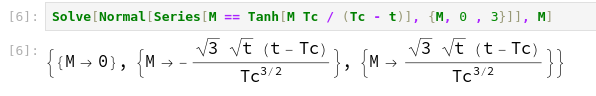
\includegraphics[scale = 0.8]{magnetization.png}
        \end{center}
        And using this in the bracketed expression of Eq~\ref{eq:crazyBracketedTerm} yields:
        \begin{align*}
          &\left(- k_B t - \frac{k_B t^2}{T_c} + M^2 B_0 + M^2 k_B t + M^2 \frac{k_B^2 t^2}{B_0}\right)\\
%          & =B_{k}  - \beta \left(1 - M^2\right) B^2_{k} &\geq 3 k_B t - 6 \frac{k_B t^2}{T_c} - k_B t + 3\frac{k_B t^2}{T_c}\\
          &\qquad = - k_B t  - \frac{k_B t^2}{T_c} + 3 k_B t - 6 \frac{k_B t^2}{T_c} + 3\frac{k_B t^2}{T_c} + \mathcal{O}(t^3)\\
          &\qquad = 2 \left(k_B t - 2 \frac{k_B t^2}{T_c} \right) + \mathcal{O}(t^3)
        \end{align*}
        Which is positive to second order in $t$ if:
        \begin{equation*}
          k_B t - 2 \frac{k_B t^2}{T_c} > 0 \Rightarrow t < \frac{T_c}{2}
        \end{equation*}
        Which is a very big bound.
        Doing the calculation to higher orders will likely make this bound tighter.
      \item
        Using the approximation:
        \begin{align*}
          S(\phi) \approx S(\psi) + \frac{1}{2}\sum_{i,j}(\phi - \psi)_i (\phi - \psi)_j \frac{\partial^2 S}{\partial \phi_i \partial \phi_j}(\psi)
        \end{align*}
        The first term is:
        \begin{align*}
          S(\psi) &= \frac{\beta}{2} (A\bar{\psi})^2 \sum_{i j} B_{ij} - \sum_i \ln(\cosh(\beta A\bar{\psi}\sum_jB_{ij}))\\
                  &= \frac{\beta}{2} M^2 \sum_{i } B_{0} - \sum_i \ln(\cosh(\beta M B_0))\\
                  &= \frac{\beta}{2} M^2 N B_{0} - N \ln(\cosh(\beta M B_0))
        \end{align*}
        And the Hessian term is:
        \begin{align*}
          \frac{1}{2}\sum_{i,j}(\phi - \psi)_i (\phi - \psi)_j \frac{\partial^2 S}{\partial \phi_i \partial \phi_j}(\psi) &= \frac{1}{2}\beta A^2 (\phi - \psi)^T B (\phi - \psi)  \\
               & \qquad   - \beta \left(1 - M^2\right) \frac{1}{2}(\phi - \psi)^T B^2 (\phi - \psi)
        \end{align*}
        And this gives the approximation for the partition function:
        \begin{align*}
          Z &\approx \sqrt{\det\left(\frac{2 \beta A^2 B}{\pi^N}\right)} \int_{\mathbb{R}^N} d^N \phi e^{-S(\psi) - (\phi - \psi) \frac{\partial S}{\partial \phi_i \partial \phi_j} (\phi - \psi)}\\
            &= \sqrt{\det\left(\frac{2^N \beta A^2 B}{\pi^N}\right)} e^{-S(\psi)}\int_{\mathbb{R}^N} d^N \phi e^{ - (\phi - \psi) \frac{\partial S}{\partial \phi_i \partial \phi_j} (\phi - \psi)}\\
            &= \sqrt{\frac{(2 \pi)^N}{\det\left( \beta A^2(B  - \beta (1 - M)^2B^2)\right)}} \sqrt{\det\left(\frac{2^N \beta A^2 B}{\pi^N}\right)} e^{-S(\psi)}\\
            &= 2^N\sqrt{\det\left(\frac{ B}{ B  - \beta (1 - M)^2B^2}\right)} e^{-S(\psi)}\\
            &= 2^N\sqrt{\det\left(\frac{ B}{ B  - \beta (1 - M)^2B^2}\right)} \exp\left[-\frac{\beta}{2} M^2 N B_{0} + N \ln(\cosh(\beta M B_0))\right]
        \end{align*}
        Which has the same form as the mean field theory parition funciton:
        \begin{align*}
          Z &\sim \sqrt{\frac{\beta qJ}{A''(x_0))}} e^{NA(x_0)}\\
            &\sim \sqrt{\frac{\beta qJ}{A''(x_0))}} e^{-N\frac{\beta q J x_0^2}{2} + N \ln(2\cosh(\beta q J x_0))}\\
            &= \sqrt{\frac{\beta qJ}{A''(x_0))}} e^{-N\frac{\beta q J x_0^2}{2} + N \ln(\cosh(\beta q J x_0)) + N \ln 2}\\
            &= 2^N\sqrt{\frac{qJ}{|-q J + \beta (1 - x_0^2) q^2 J^2 |}} e^{-N\frac{\beta q J x_0^2}{2} + N \ln(\cosh(\beta q J x_0))}
        \end{align*}
        With $B \sim qJ$ and $x_0 \sim M$.
      \item
        The integral in the denominator is:
        \begin{align*}
          \int_{\mathbb{R}^N} d^N\phi \exp\left[-\frac{\beta A^2}{2}(\phi - \psi)^T\left(B  - \beta (1 - M^2)B^2)\right) (\phi - \psi)\right]
        \end{align*}
        The integral is invariant under the change of variables $\tilde\phi = \phi - \psi$:
        \begin{align*}
          &\int_{\mathbb{R}^N} d^N\tilde\phi \exp\left[-\frac{\beta A^2}{2}\tilde\phi^T\left(B  - \beta (1 - M^2)B^2\right) \tilde\phi\right]\\
          & \qquad = \sqrt{\frac{(2 \pi)^N}{\det\left( B  - \beta (1 - M)^2B^2\right)}}
        \end{align*}
        And the integral in the numerator under the same change of variables is:
        \begin{align*}
            &\int_{\mathbb{R}^N} d^N\phi \exp\left[-\frac{\beta A^2}{2}\tilde\phi^T\left(B  - \beta (1 - M^2)B^2)\right) \tilde\phi \right] (\tilde \phi_i + \psi_i)\\
          = & \int_{\mathbb{R}^N} d^N\phi \exp\left[-\frac{\beta A^2}{2}\tilde\phi^T\left(B  - \beta (1 - M^2)B^2)\right) \tilde\phi \right]\psi_i\\
          = & \psi_i\int_{\mathbb{R}^N} d^N\phi \exp\left[-\frac{\beta A^2}{2}\tilde\phi^T\left(B  - \beta (1 - M^2)B^2)\right) \tilde\phi \right]\\
          = & \psi_i \sqrt{\frac{(2 \pi)^N}{\det\left( B  - \beta (1 - M)^2B^2\right)}}
        \end{align*}
        The integral with $\tilde \phi$ not in the exponent is the integral of an odd times an even function so is zero.
        Putting these two together:
        \begin{equation*}
          \langle \sigma_i \rangle \approx A \frac{\psi_i \sqrt{\frac{(2 \pi)^N}{\det\left( B  - \beta (1 - M)^2B^2\right)}}}{\sqrt{\frac{(2 \pi)^N}{\det\left( B  - \beta (1 - M)^2B^2\right)}}} = A \bar{\psi} = M
        \end{equation*}
        And the average magnetization is:
        \begin{equation*}
          M_{\text{avg}} = \frac{1}{N} \sum_{i} \langle \sigma_i \rangle = \frac{1}{N} \sum_{i} M = \frac{1}{N} NM = M
        \end{equation*}
        The beta critical exponent is given by Eq~\ref{eq:magnetization} repeated here after some rearranging:
        \begin{equation}
          M \approx \pm \sqrt{3} \left(\frac{|T - T_c|^{1/2}}{T_c^{1/2}} \right) 
        \end{equation}
        so that $\beta = 1/ 2$.
      \item
        I am not sure what is meant by exact result here. I presume it is not refering to the exact solution of the Ising model, which has no known exact solution in 3D.
        Either way, the approximation in this calculation does not get better with increasing $N$ for the simple reason that there is no $N$ appearing in the Gaussian integral:
        \begin{align*}
          &\int_{\mathbb{R}^N} d^N \phi \exp[ - (\phi - \psi) \frac{\partial S}{\partial \phi_i \partial \phi_j} (\phi - \psi)]\\
          &\qquad= \qquad \int_{\mathbb{R}^N} d^N \phi \exp[ - \frac{1}{2}(\phi - \psi)^T 
          \left(
\beta A^2  B \left(1 - M^2\right)  B^2\right) (\phi - \psi)]
        \end{align*}
        This Gaussian integral here does not get any more dominant, taller and sharper, as $N$ increases so the approximation made above in calculating the partition funciton is no more exact.
        This is quite different from the use of Laplace's method where the $N$ in the exponent of the integral makes the Gaussian function sharper and taller; therefore, it makes the integral's approximation more accurate.
        The above approximation holds for smaller $N$, whereas Laplace's method only works for very large N.
    \end{enumerate}
\end{enumerate}
\end{document}
